%% This is file `elsarticle-template-1-num.tex',
%%
%% Copyright 2009 Elsevier Ltd
%%
%% This file is part of the 'Elsarticle Bundle'.
%% ---------------------------------------------
%%
%% It may be distributed under the conditions of the LaTeX Project Public
%% License, either version 1.2 of this license or (at your option) any
%% later version.  The latest version of this license is in
%%    http://www.latex-project.org/lppl.txt
%% and version 1.2 or later is part of all distributions of LaTeX
%% version 1999/12/01 or later.
%%
%% Template article for Elsevier's document class `elsarticle'
%% with numbered style bibliographic references
%%
%% $Id: elsarticle-template-1-num.tex 149 2009-10-08 05:01:15Z rishi $
%% $URL: http://lenova.river-valley.com/svn/elsbst/trunk/elsarticle-template-1-num.tex $
%%
%\documentclass[preprint,12pt]{elsarticle}

%% Use the option review to obtain double line spacing
\documentclass[preprint,review,12pt]{elsarticle}

%% Use the options 1p,twocolumn; 3p; 3p,twocolumn; 5p; or 5p,twocolumn
%% for a journal layout:
%% \documentclass[final,1p,times]{elsarticle}
%% \documentclass[final,1p,times,twocolumn]{elsarticle}
%% \documentclass[final,3p,times]{elsarticle}
%% \documentclass[final,3p,times,twocolumn]{elsarticle}
%% \documentclass[final,5p,times]{elsarticle}
%% \documentclass[final,5p,times,twocolumn]{elsarticle}

%% The graphicx package provides the includegraphics command.
\usepackage{graphicx}
%% The amssymb package provides various useful mathematical symbols
\usepackage{amssymb}
%% The amsthm package provides extended theorem environments
%% \usepackage{amsthm}

%% The lineno packages adds line numbers. Start line numbering with
%% \begin{linenumbers}, end it with \end{linenumbers}. Or switch it on
%% for the whole article with \linenumbers after \end{frontmatter}.
\usepackage{lineno}
\usepackage{ragged2e}
\usepackage{gensymb}
\usepackage{wasysym}
\usepackage{amsmath}
\usepackage{hyperref} % Hyperlinks
\usepackage{placeins} %  Used for graphics placement
\usepackage{natbib}
\setcitestyle{round,authoryear}

\hypersetup{colorlinks,linkcolor=black,urlcolor=blue}


%% natbib.sty is loaded by default. However, natbib options can be
%% provided with \biboptions{...} command. Following options are
%% valid:

%%   round  -  round parentheses are used (default)
%%   square -  square brackets are used   [option]
%%   curly  -  curly braces are used      {option}
%%   angle  -  angle brackets are used    <option>
%%   semicolon  -  multiple citations separated by semi-colon
%%   colon  - same as semicolon, an earlier confusion
%%   comma  -  separated by comma
%%   numbers-  selects numerical citations
%%   super  -  numerical citations as superscripts
%%   sort   -  sorts multiple citations according to order in ref. list
%%   sort&compress   -  like sort, but also compresses numerical citations
%%   compress - compresses without sorting
%%
%% \biboptions{comma,round}

% \biboptions{}

\journal{Estuarine, Coastal, and Shelf Science}

\begin{document}

\newcommand\fnurl[2]{%
\href{#1}{#2}\footnote{\url{#1}}%
}

\begin{frontmatter}
\RaggedRight
%% Title, authors and addresses

\title{Implications of Shifting Stratification Dynamics on Phytoplankton Blooms in San Francsico Bay Under Future Scenarios}

%% use the tnoteref command within \title for footnotes;
%% use the tnotetext command for the associated footnote;
%% use the fnref command within \author or \address for footnotes;
%% use the fntext command for the associated footnote;
%% use the corref command within \author for corresponding author footnotes;
%% use the cortext command for the associated footnote;
%% use the ead command for the email address,
%% and the form \ead[url] for the home page:
%%
%% \title{Title\tnoteref{label1}}
%% \tnotetext[label1]{}
%% \author{Name\corref{cor1}\fnref{label2}}
%% \ead{email address}
%% \ead[url]{home page}
%% \fntext[label2]{}
%% \cortext[cor1]{}
%% \address{Address\fnref{label3}}
%% \fntext[label3]{}


%% use optional labels to link authors explicitly to addresses:
%% \author[label1,label2]{<author name>}
%% \address[label1]{<address>}
%% \address[label2]{<address>}

\author{Emma Nuss, Dave Senn, Derek Roberts, others?}

%\address{California, United States}

%\begin{abstract}
%% Text of abstract

%\end{abstract}

\begin{keyword}

%% keywords here, in the form: keyword \sep keyword

%% MSC codes here, in the form: \MSC code \sep code
%% or \MSC[2008] code \sep code (2000 is the default)

\end{keyword}

\end{frontmatter}

%%
%% Start line numbering here if you want
%%
\linenumbers

%% main text
\section{Introduction}\label{S:intro}
Eutrophication frequently occurs in estuarine and shallow coastal environments where an excess of nutrients runoff, fueling increased algal growth, and leading to low dissolved oxygen levels. San Francisco Bay (SFB) is an urbanized estuary with high nutrient loads from agricultural and stormwater runoff and wastewater treatment plant (WWTP) discharge. Wastewater discharge provides the largest proportion (65\%) of nutrient loads to the estuary, with runoff from agriculture via the Sacramento-San Joaquin River Delta making up 20\% and local storm-water runoff making up 15\% \citep{novick2014}. Despite these high nutrient loads and high ambient nutrient concentrations within SFB, spring chlorophyll blooms are not consistently large and have strong inter-annual variability (cite**). 

Previous work has shown that high turbidity and benthic grazers can exhibit controls on phytoplankton growth (cite**). For example, in the north part of SFB, an invasive clam species (\textit{Corbicula fluminea}) strongly modulates phytoplankton biomass \citep{lucas2002, lopez2006}. Additionally, throughout the Bay, suspended sediment concentrations can limit light availability, inhibiting phytoplankton growth. The photic zone in San Francisco Bay is typically ** meters, but varies over numerous timescales (cite**).  

The effect of suspended sediment and benthic grazers are both modulated by the strength of stratification of the water column. Stronger stratification allows phytoplankton to spend more time in the upper part of the water column, increasing the light levels they experience and their distance from benthic grazers. Phytoplankton blooms in South SFB have been observed to be associated with stratification \citep{cloern1991}. Stratification in tidal estuarine environments are controlled by horizontal salinity gradients set up through freshwater flows to the estuary. The salinity gradient and the effect of tides on this gradient can create periodic stratification known as strain-induced periodic stratification (SIPS) \citep{simpson1990}. When the salinity gradient is strong enough and tidal mixing is weak enough, SIPS can set up vertical stratification which can persist through multiple tidal cycles, given the right conditions. Stratification that persists through multiple tidal cycles provides phytoplankton ideal growth conditions. Prolonged stratification decreases the depth of the mixed layer and ensures that phytoplankton are exposed to higher light levels. 

While stratification has been shown to be an important control on phytoplankton growth in SFB, the relationship has not been fully quantified and the relationship between stratification and phytoplankton growth is not predictive. Northern California precipitation projections predict increases in extreme wet and dry years, as well as increases in sub-seasonal storms \citep{swain2018}). This change in precipitation patterns will affect the distribution of salinity in SFB and, in turn, stratification dynamics. Quantifying the relationship between stratification and chlorophyll and developing predictive capability would be instrumental in understanding future ecological conditions in SFB and assist in making management decisions that would affect the health of the bay. 

In this study we focus on South SFB, which exhibits the highest ambient nutrient concentrations \citep{novick2014}. In addition to high nutrient concentrations, this subembayment has longer residence times than any other part of the bay. High nutrient concentrations, in conjunction with long residence times, provide a system that could be susceptible to low dissolved oxygen concentrations and poor ecological conditions. We aim to understand South SFB's susceptibility to eutrophication conditions under changes in freshwater flow and shifts in stratification dynamics.

This study makes use of the long-term water quality dataset collected by USGS along the transect of SFB and a hydrodynamic model developed for SFB. It is hypothesized that sustained stratification events could lead to increased chlorophyll levels. We aim to quantify the importance of stratification in observed chlorophyll using this long-term dataset and use a probabilistic approach to estimate a relationship. We use this relationship and the hydrodynamic model to predict the effect of various freshwater flow conditions on chlorophyll conditions in South SFB, and how these could act as proxies for future climate scenarios.  

\section{Methods}\label{S:methods}
\subsection{Data}\label{S:data}
Data sets of South Bay salinity, stratification, tidal velocity, freshwater flow, and chlorophyll were compiled and used to understand the effect of environmental conditions on chlorophyll observations. United States Geological Survey (USGS) Alameda Creek (USGS Station 11179000) daily flow data was used for an estimate of South Bay freshwater flow conditions. National Oceanic and Atmospheric Administration (NOAA) acoustic doppler current profiler (ADCP) data at San Mateo Bridge was harmonically decomposed and used to create tidal velocity predictions for the desired time record. Salinity and chlorophyll data from USGS bi-monthly cruises were compiled for South Bay stations (22 - 32).  

To quantify the relationship between chlorophyll and environmental conditions, we utilize the data to complete a conditional probabilistic analysis of the likelihood of chlorophyll given various conditions. This analysis required data to be on a synchronous time interval. Raw data was available on a number of different timescales, from bi-monthly to sub-daily, and as such, different mechanisms were used to create daily records. Tidal velocity data was sub-sampled from hourly to daily by extracting the daily maximum flood velocity. **?**Depth averaged salinity data at South Bay stations were interpolated through time using a generalized additive model (***details from Dave). This interpolated salinity data was used to calculate daily horizontal salinity gradient metrics. Raw salinity data was used to calculate stratification only for the days available and was left masked on days with no data. Similarly, chlorophyll data was kept as raw data for available days and freshwater flow data already was given as daily flow. The final version of this processed data set included daily maximum flood velocity at San Mateo Bridge, daily interpolated longitudinal salinity gradient between South Bay USGS cruise stations (22-32), daily flow at Alameda Creek, and stratification and chlorophyll at South Bay USGS cruise stations (22-32) for available days. 

The horizontal Richardson number (\(Ri_x\)) was calculated from daily salinity gradient and tidal velocity data as a vertical stratification metric. \(Ri_x\) is a metric that captures the balance between the stratifying forces of tidal straining and the destratifying forces of tidal mixing and is defined as:
\begin{equation}
    Ri_x = \frac{\beta g \frac{ds}{dx} H^2}{u_*^2}
\end{equation}
where \(\frac{ds}{dx}\) is the horizontal salinity gradient, \(H\) is the water depth, \(g\) is gravity, \(\beta\) is the saline contraction coefficient, and \(u_*\) is the friction velocity. \(Ri_x\) was calculated for each day in the data range using mean water depth, 10\% of the daily maximum flood velocity as an approximation for friction velocity (\(u_* = 0.1 u_{tidal}\)), and the depth-averaged horizontal salinity gradient between USGS station 27 and 32. 

\subsection{Probabilistic Analysis}
A probabilistic approach was taken to analyze the data. The calculated \(Ri_X\) and observed chlorophyll was used to calculate pseudo-conditional probability distributions of the likelihood of observing chlorophyll for a given \(Ri_x\). To do this, we first applied a 3-day backwards-looking window to the daily \(Ri_x\) and selected the minimum value in that window to produce a minimum \(Ri_x\) time series. Next, quantile ranges were chosen to apply to \(Ri_x\), binning the coinciding observations into each respective quantile range. For each \(Ri_x\) quantile range, the coincident chlorophyll data points were subset. From this, the chlorophyll observations were further subdivided into chlorophyll quantile ranges. The probability of observing chlorophyll of a given quantile or higher was calculated from the subset of chlorophyll data by computing the frequency of observations in which the subset of chlorophyll observations exceeded the quantile range threshold and then divided by the total number of observations of the subset of chlorophyll. This process was repeated for each \(Ri_x\) quantile & chlorophyll quantile pair, creating a 2-dimensional probability map. 

These probability calculations result in gridded data of the probability of observing chlorophyll above a chosen chlorophyll quantile, given a minimum quantile of \(Ri_x\) in the 3 days prior to the observation. This gridded data can be converted to a continuous function, which can be used to estimate the probability of exceeding a given chlorophyll quantile for any given \(Ri_x\) quantile. This continuous function is achieved through the use of radial basis functions. The general form of a radial basis function is: 
\begin{equation}\label{eq:rbf}
    s(\vec{x}) = \sum \alpha_i \Phi_i ( |\vec{x} - \vec{x_i}|),
\end{equation}
where \(\alpha_i\) are weights (estimated through least squares), \(\Phi_i\) are the basis functions, \(\vec{x}\) is the coordinate location (i.e., the given chlorophyll and Ri\(_x\) pairs), and \(\vec{x_i}\) are the reference locations of known values. 
The chosen form of the basis function is a polyharmonic spline of the form:
\begin{equation}\label{Phi}
    \Phi (r) = r^2 \ln(r).
\end{equation}
For our setup, \(r = \vec{x} - \vec{x_i}\), indicating that the radial distance is measured as the distance from given chlorophyll (\(q_{chl}\)) and \(Ri_x\) quantiles (\(q_{Ri_x}\)) from the reference quantiles used in the probability calculations from observations:
\begin{equation}\label{eq:distance}
    r(q_{chl}, q_{Ri_x}) = \sqrt{(q_{chl}-q_{chl}(i))^2 + (q_{Ri_x}-q_{Ri_x}(i))^2}
\end{equation}
The result is a function (\(s(q_{chl}, q_{Ri_x})\)) that calculates probability given a choice of chlorophyll quantile threshold (\(q_{chl}\)) and a \(Ri_x\) quantile (\(q_{Ri_x}\)):
\begin{equation}\label{eq:full_rbf}
    s(q_{chl}, q_{Ri_x}) = \sum \alpha_i \Phi_i ( r(q_{chl}, q_{Ri_x})).
\end{equation}

\subsection{Hydrodynamic Model}\label{S:model}
To explore realistic hydrodynamic conditions under various freshwater flow conditions we utilize a hydrodynamic model that is set up and calibrated for SFB. The hydrodynamic model is built on {\em D-Flow Flexible Mesh} (DFM), a finite-volume, three-dimensional, unstructured hydrodynamic model \citep{martyr2017}. The original model setup was developed and outlined in \cite{pubben2017} as a part of the USGS Computational Assessments of Scenarios of Change for the Delta Ecosystem (CASCaDE) and San Francisco Bay-Delta Community Model projects. The most pertinent model details are given below; however, a full description of hydrodynamic model setup and validation of performance can be found in \cite{holleman2017}. 

\subsubsection{Model Grid}
The model is an unstructured horizontal grid with sigma vertical levels. The model grid encompasses SFB and extends into the coastal ocean, from approximately 20 km off of Point Reyes in the north-west corner and 40 km west of Half Moon Bay in the southwest corner, roughly covering the San Francisco Bight (Fig. \ref{fig:grid}). Horizontal grid resolution varies from fine scale resolution (~20 m) in shallow slough areas to over 2 km in the offshore, for a total of 49,996 grid cells. Nominal resolution for areas of interest are between 250 m (South SFB) and 350 - 500 m (North SFB). In the vertical, there are 10 sigma layers, with varying layer thickness in relation to water depth. 

Bathymetry is prescribed at the nodes of each grid cell from linear interpolation of 10 m topo-bathymetry from California Department of Water Resources \citep{wang2012} and high-resolution USGS bathymetry in Lower South Bay \citep{foxgrover2018}. Elevation data are relative to the NAVD88 vertical datum. 

\begin{figure}[ht!]
\centering
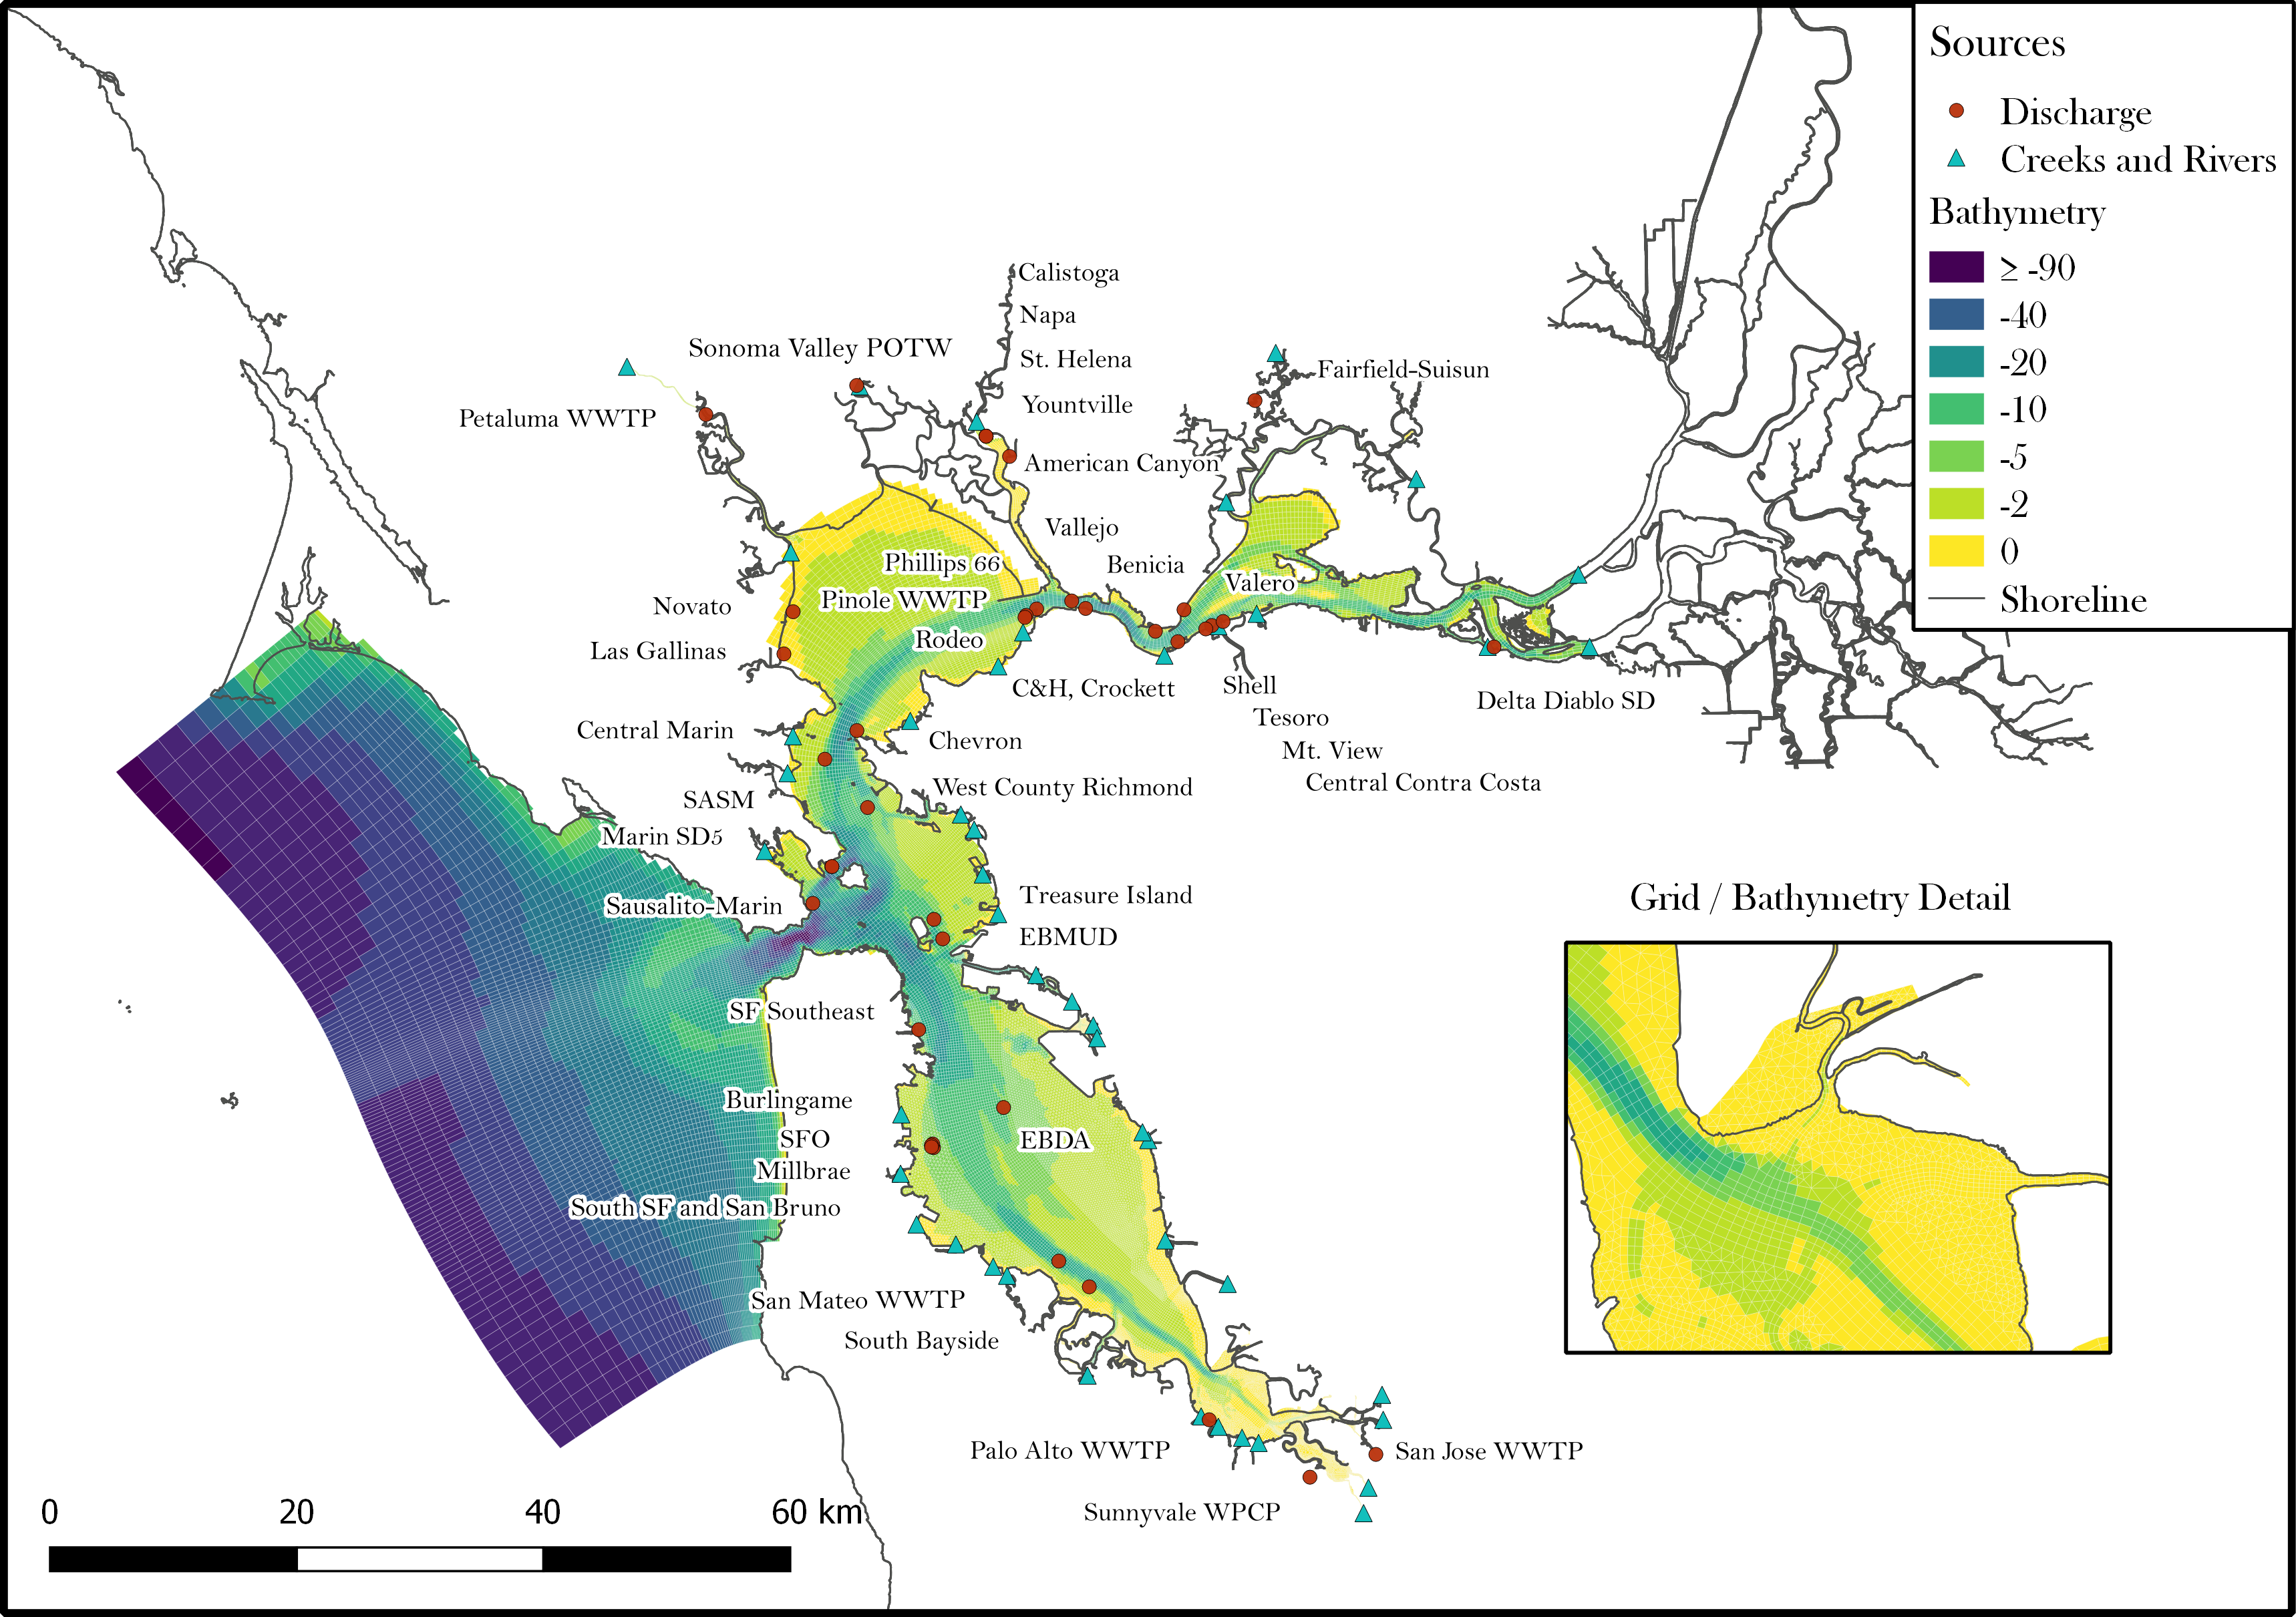
\includegraphics[width=\textwidth]{Figures/grid_inputs_v21.png}
\caption{San Francisco Bay DFM grid}
\label{fig:grid}
\end{figure}
\FloatBarrier

\subsubsection{Boundary Conditions}
The open ocean boundary is tidally forced with observed 6-minute water level data (NOAA gage 9415020) and salinity and temperature are set to 33 ppt and *** respectively. Water level forcing data is is low-pass filtered with a 4th-order Butterworth filter with a 3-hour cutoff period. The shorter northern and southern edges of the ocean boundary are closed.

Freshwater flows were derived from the Bay Area Hydrologic Model (a HSPF-based hydrologic model**cite?), calibrated against gage data over the 2000–2016 period. This model includes ***check this number*** 44 separate river and stormwater inputs to SFB (Fig. \ref{fig:grid}). All river and stormwater inputs are assumed to enter the Bay with negligible salinity (i.e. 0 ppt) and constant temperature of 20\(\degree\)C.

The edge of the model domain is at Rio Vista on the Sacramento River, and Jersey Point on the San Joaquin River. Boundary conditions here are taken from USGS streamflow gages (11455420 and 11337190 for the Sacramento and San Joaquin flows, respectively). Salinity is negligible and set accordingly, while water temperature is obtained from the same USGS gaging stations and assigned to in-flowing water in the model. 

Wastewater treatment plants (WWTPs) inputs can be significant freshwater sources and influence the density field. Flow and load data for 37 WWTPs and 5 refineries are used as inflows to the bay. For dates when flow data is unavailable, a flow rate is estimated based on inter-annual trends and a seasonal flow climatology. Each of the 42 inflows have been added to the hydrodynamic model as a freshwater source located at the bed.

The wind field is interpolated from 52 wind stations around SFB and specified hourly on a 1.5 km by 1.5 km grid. Specifics of the interpolation method and data sources can be found in King (2019) **cite**. 

In addition to stormwater runoff, which enters the model at prescribed locations along the boundary, we also include direct precipitation and evaporation acting directly on the water surface. The model incorporates measured precipitation and evapotranspiration (ET\degree) from the CIMIS Union City station. 

\section{Results}\label{S:results}

\subsection{Probabilistic Analysis}
Our probabilistic analysis relies heavily on the calculated stratification metric, \(Ri_x\). This metric is compared to the cruise-averaged stratification profiles from USGS stations 24, 25, 27, and 29. Multiple stations were averaged together to minimize noise from any one station's variability and also to compare how \(Ri_x\) captures the aggregate stratification condition in this region of the bay. USGS cruises sample at various phases in the tidal cycle and thus the observed stratification may at times be biased by ebb tide stratification due to tidal straining; however, \(Ri_x\) tends to agree well with observed stratification (Fig. \ref{fig:rix}). Times of observed strong stratification correspond well with higher \(Ri_x\).

\begin{figure}[ht!]
\centering
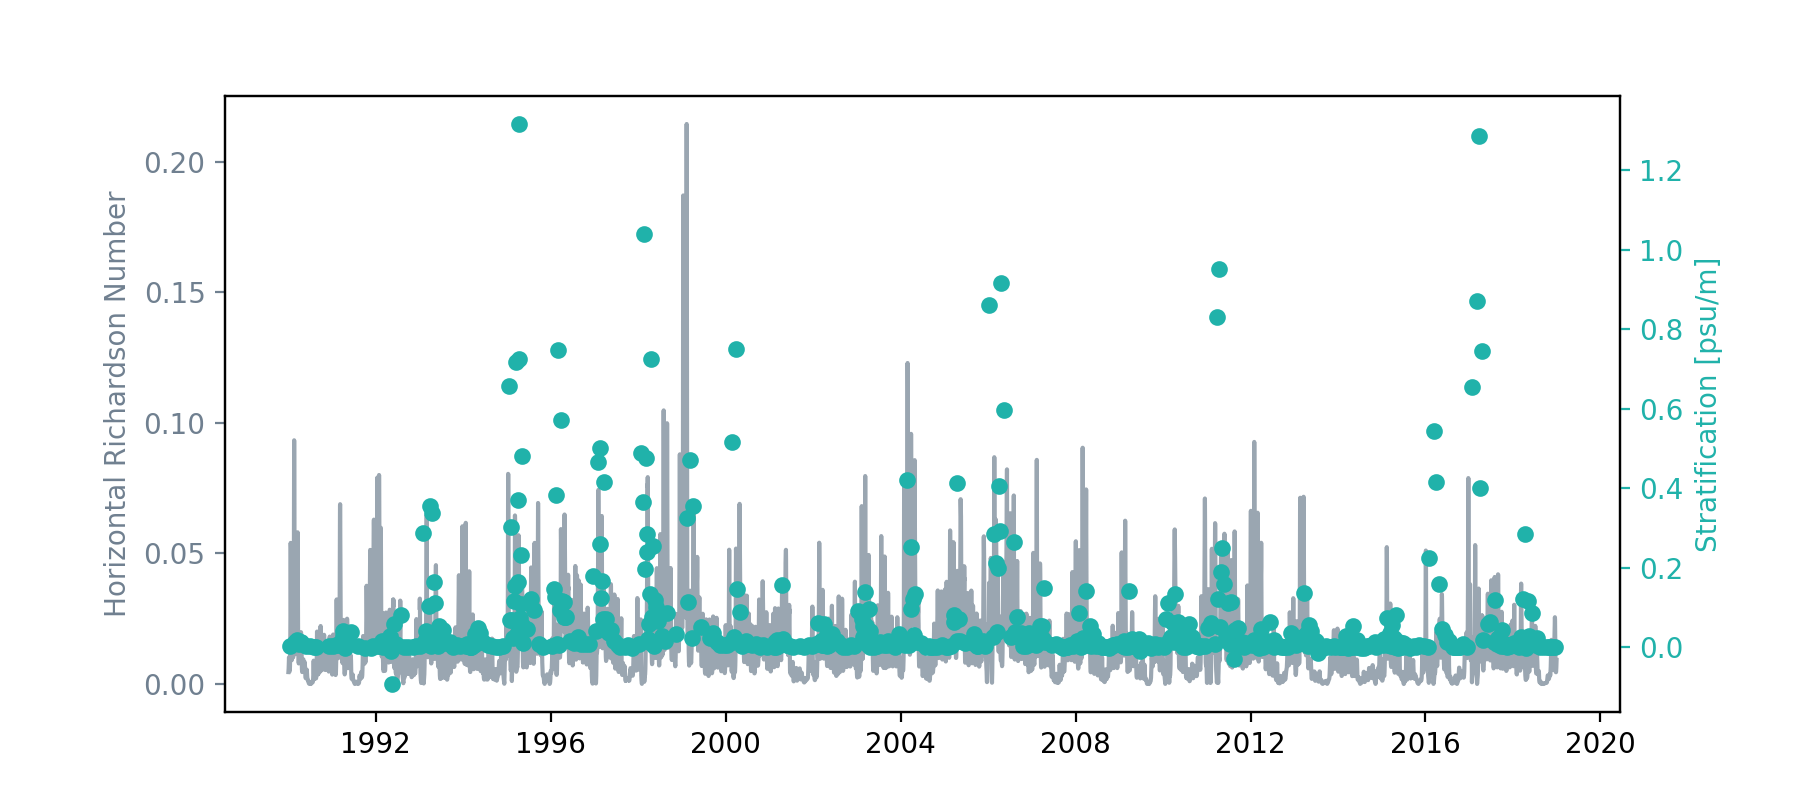
\includegraphics[width=\textwidth]{Figures/Rix_dsdz_timeseries.png}
\caption{Calculated daily horizontal Richardson number and observed stratification averaged between USGS stations 24, 25, 27, and 29}
\label{fig:rix}
\end{figure}
\FloatBarrier

Ten quantile bins evenly spaced between 0 and 1 were defined for \(Ri_x\) in bin sizes of 0.1. Chlorophyll observations were subset by the corresponding 3-day windowed \(Ri_x\). The number of observations (n-value) for each chlorophyll subset hovered around 55 for each \(Ri_x\) quantile bin. The probability of observing chlorophyll at greater than or equal to a particular chlorophyll threshold was calculated for each chlorophyll subset using varying chlorophyll quantile thresholds from 0.1 to 0.9. The contours in Figure \ref{fig:chl_pdf} show the results of these calculations. The probability of observing a chlorophyll level of 0.1 quantile or higher is around 0.9-1.0 for all quantiles of \(Ri_x\), indicating a very high likelihood that the chlorophyll level could exceed this very low threshold. Likewise, as the chlorophyll threshold is increased in the probability calculation, probabilities drop rapidly resulting in their minimum values at the highest chlorophyll threshold (quantile 0.9) ranging from approximately 0 to 0.18 the \(Ri_x\) quantile increases. Probabilities generally increase as you increase \(Ri_x\) and decrease as you increase chlorophyll quantile. These results support the hypothesis that more stratification can lead to increased likelihood of high chlorophyll levels.

\begin{figure}[ht!]
\centering
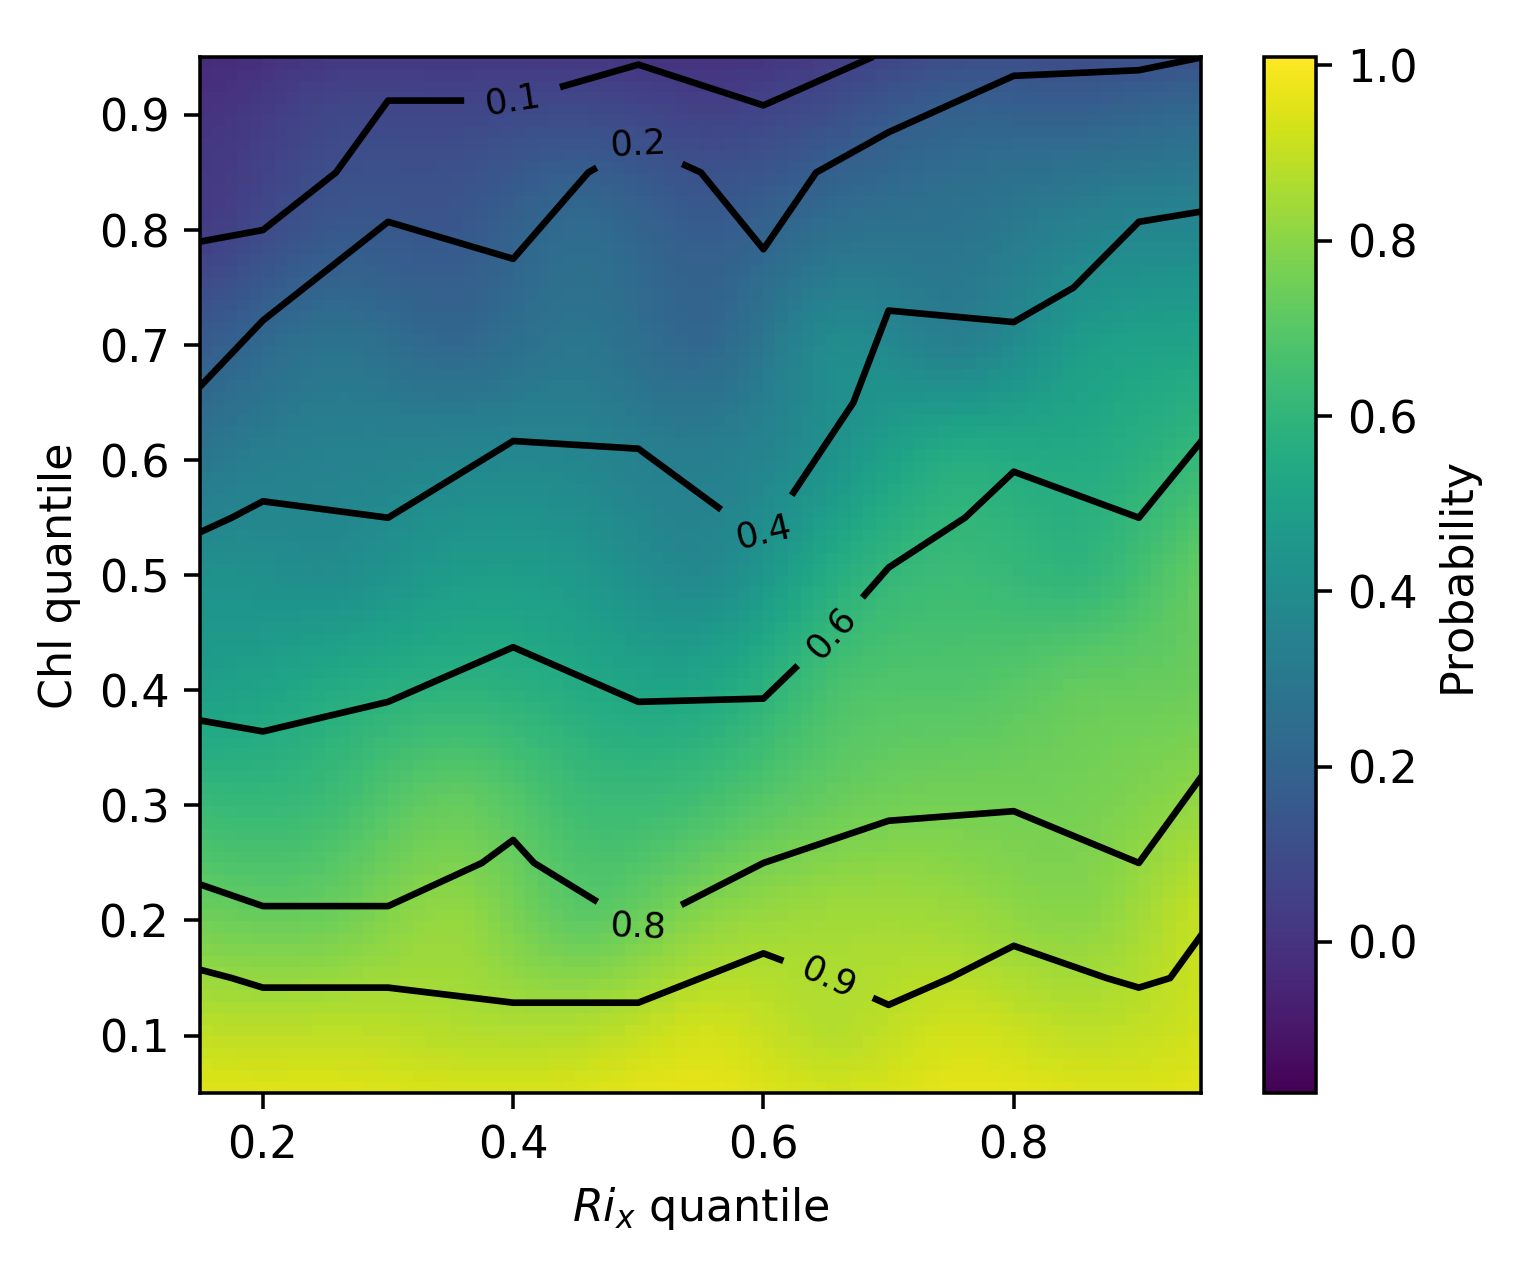
\includegraphics[width=\textwidth]{Figures/chl_rix_rbf_pdf.png}
\caption{Probability of observing chlorophyll of the corresponding chlorophyll quantile or higher given the observed \(Ri_x\) quantile in the 3 days prior. Contours indicate the results directly from observations. Shading displays these same calculated probabilities, but calculated with equation \ref{eq:full_rbf} for finer resolution.}
\label{fig:chl_pdf}
\end{figure}
\FloatBarrier

Equation \ref{eq:full_rbf} was used to create a continuous function from the calculated probabilities. The results are shown in Figure \ref{fig:chl_pdf}, where the contours show the calculated probabilities directly from the data, while the shading shows the probabilities calculated via equation \ref{eq:full_rbf}. Equation \ref{eq:full_rbf} captures the data well, and allows for calculation of probabilities for any set of chlorophyll and \(Ri_x\) quantiles. This capability is utilized with the model calculated \(Ri_X\) from hydrodynamic model output. 

\subsection{Hydrodynamic Simulation}
The hydrodynamic model was run from August 2012 through September 2013 (Water Year 2013) and from August 2016 through September 2017 (Water Year 2017). For both runs, August through September were used as a two month spin up period. Validation of water level, velocity, temperature, and salinity for available locations and times provide good agreement. A detailed validation of the model setup is found in \cite{holleman2017}). 

Water year 2013 and 2017 were chosen for simulation because the flow conditions observed in both years served as observational extremes. Water year 2013 was a low flow year in the midst of a state-wide drought. Conversely, 2017 was an extremely wet year. These two years provide an interesting comparison of stratification conditions in San Francisco Bay and provide proxies for projected future conditions.  

To analyze the model output, \(Ri_x\) was calculated in a similar manner as the observations used the probabilistic analysis. \(Ri_x\) was calculated as the distance normalized salinity difference between the approximate locations of San Mateo Bridge and Dumbarton Bridge in the model grid. This horizontal salinity gradient data was down-sampled to daily data by taking the average over each day. Depth-averaged tidal velocity data was taken at San Mateo Bridge and down-sampled to daily data by taking the daily maximum flood velocity. Water depth data was taken at San Mateo Bridge and down-sampled to daily data by taking the day average water depth. The daily \(Ri_x\) was calculated from the modeled data by the same method described in Section \ref{S:data}.

Distributions of \(Ri_x\) from observations, water year 2013, and water year 2017 are compared in Figure \ref{fig:rix_hist}. The following statistical calculations are performed for a log distribution. The distribution of observation calculated \(Ri_x\) has a mean of -2.0 and a standard deviation of 0.5. The range of the observed distribution is from -4.9 to -1.0. The model calculated \(Ri_x\) for water year 2013 has a mean of -2.2 and a standard deviation of 0.5. The range of the water year 2013 distribution is -4.4 to -1.2. For water year 2017, the mean is -1.8 and the standard deviation is 0.4. The range of the distribution is from -3.3 to -0.6. These distributions match with expectations, where the observed \(Ri_x\) distribution is relatively log normally distributed spanning roughly the same range as both water year 2013 and 2017. The distribution of water year 2017, an extreme wet year, is shifted towards stronger \(Ri_x\) as would be expected and conversely water year 2013 is shifted towards weaker \(Ri_x\). 

\begin{figure}[ht!]
\centering
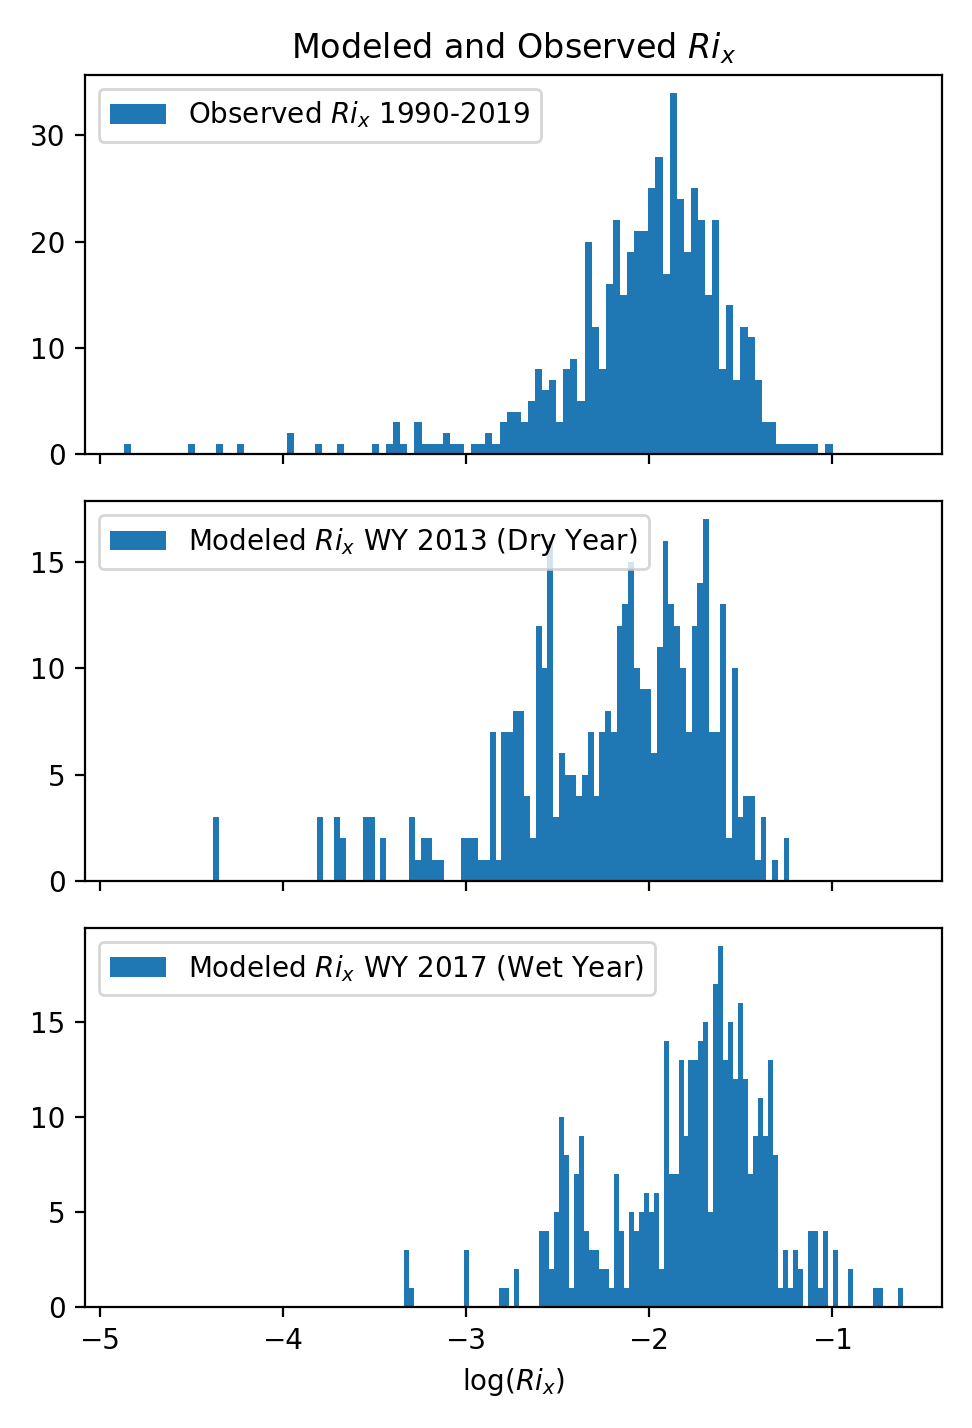
\includegraphics[width=0.8\textwidth]{Figures/rix_hist.png}
\caption{Histograms of daily 3-day windowed \(Ri_x\), as calculated from observations, water year 2013 model output, and water year 2017 model output.}
\label{fig:rix_hist}
\end{figure}
\FloatBarrier

To use equation \ref{eq:full_rbf} with the model conditions, the model calculated \(Ri_x\) are converted to an equivalent quantile from within the observation calculated distribution. Figure \ref{fig:quant_hist} shows the distribution of the quantiles for both model years and observations. As expected, observation quantiles are evenly distributed between 0 and 1; however, the histograms of water year 2013 and 2017 show different distributions. Water year 2013 has a higher frequency of low quantiles, whereas, water year 2017 has a high frequency of high quantiles (Fig. \ref{fig:quant_hist}). These quantile distributions are consistent with the \(Ri_x\) distribution statistics and the conditions observed in each year. 

\begin{figure}[ht!]
\centering
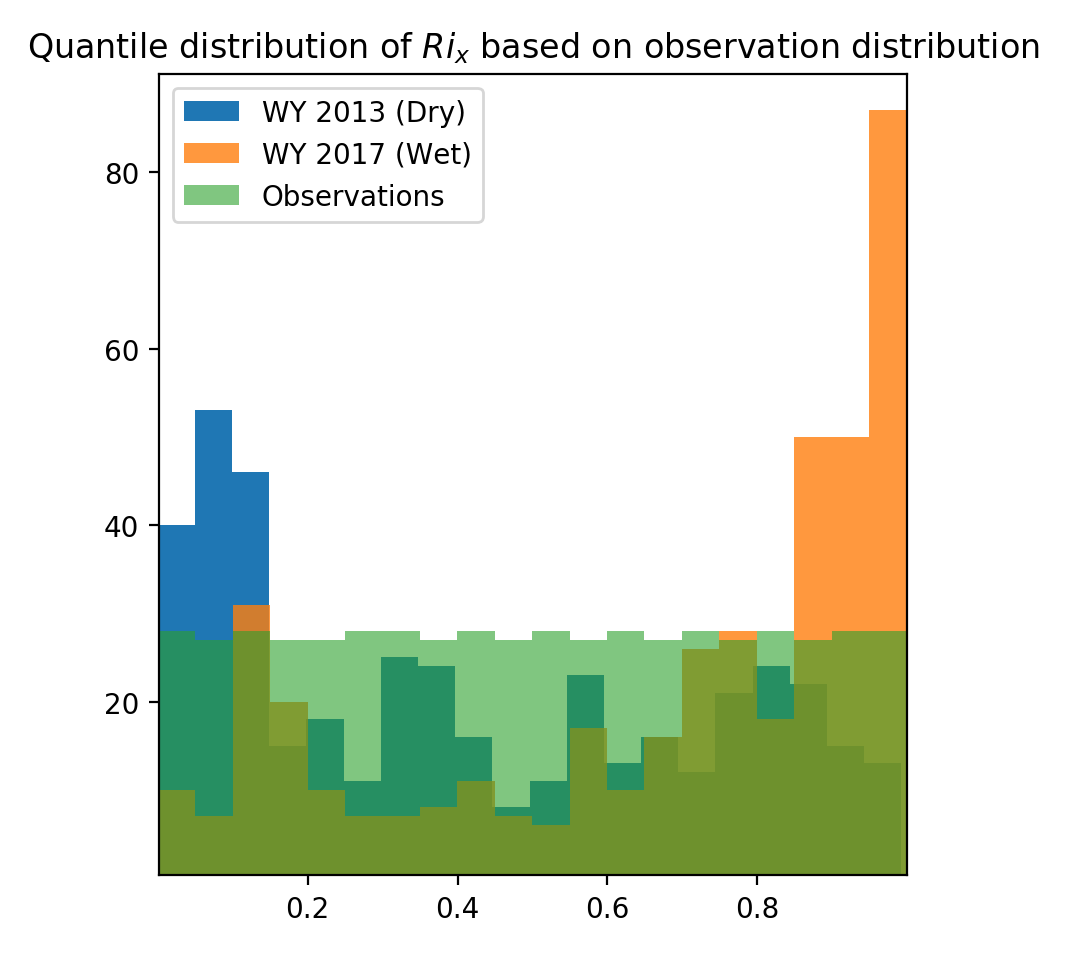
\includegraphics[width=0.7\textwidth]{Figures/quantile_rix_dist.png}
\caption{Histogram of number of \(Ri_x\) values in each quantile of the observation calculated distribution of \(Ri_x\). Green bars indicate the observation \(Ri_x\) distribution, as seen by being nearly evenly distributed across all quantiles. Water year 2013 is indicated by the blue bars, and water year 2017 is indicated by the orange bars.}
\label{fig:quant_hist}
\end{figure}
\FloatBarrier

The \(Ri_x\) time series from both water year model runs were used to create a time series of probabilities, using equation \ref{eq:full_rbf}. Three chlorophyll quantile thresholds (0.5, 0.75, 0.9) were used calculate this time series for each model run. These quantile thresholds correspond to chlorophyll levels of 4.5, 6.9, and 13.8 \(mg/m^3\). 

Across all three chlorophyll thresholds, water year 2017 has a pattern of more prolonged and higher probabilities of observing the given chlorophyll quantile than water year 2013. Probabilities are highest, in both years, for observing chlorophyll greater than the 0.5 quantile. Probabilities are more consistently high through spring and into summer in water year 2017, whereas water year 2013 probabilities drop significantly by June. If the probability of exceeding a quantile (\(q\)) were a random variable, then the expected probability (\(p\)) is \(p=1-q\). For example for a quantile of 0.75, the expected probability is 0.25. Interestingly, in spring 2017, for all 0.5, 0.75 and 0.9 quantile thresholds, the probaility of observing those events given the \(Ri_x\) conditions is increased above expected likelihood. There are periods in 2013 that exceed the expected likelihood as well, but are much fewer in frequency and length.

\begin{figure}[ht!]
\centering
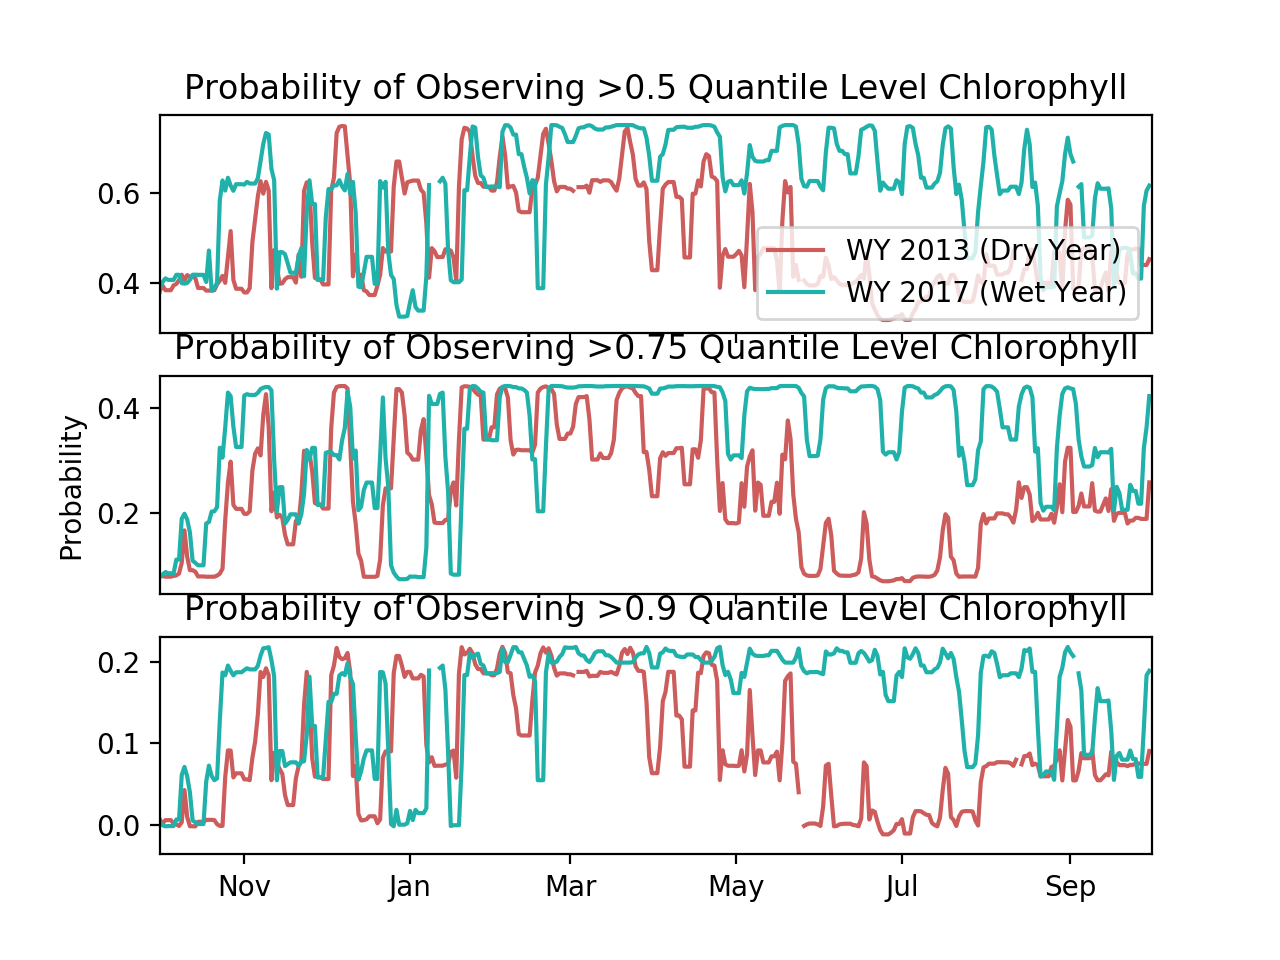
\includegraphics[width=0.8\textwidth]{Figures/probability_chl_levels_wy13_wy17.png}
\caption{Probability of observing chlorophyll greater than the 0.5, 0.75, and 0.9 chlorophyll quantile, as calculated using the modeled daily 3-day windowed \(Ri_x\) for both water year 2013 and 2017.}
\label{fig:prob_levels}
\end{figure}
\FloatBarrier

The calculated probabilities correspond well with observed chlorophyll in South Bay. Average chlorophyll levels at South Bay USGS stations (24, 25, 27, and 29) are shown with calculated probabilities in Figure \ref{fig:chl_comp}. Observed chlorophyll levels exceed the 0.75 quantile threshold in spring 2017, which corresponds to a period of elevated probabilities. While spring 2013 chlorophyll observations do not exceed the 0.75 quantile, they nonetheless are elevated, corresponding well with elevated probabilities; however, chlorophyll levels are also elevated in July 2013 and probabilities are quite low and could be indicative of additional processes important to phytoplankton production. 

\begin{figure}[ht!]
\centering
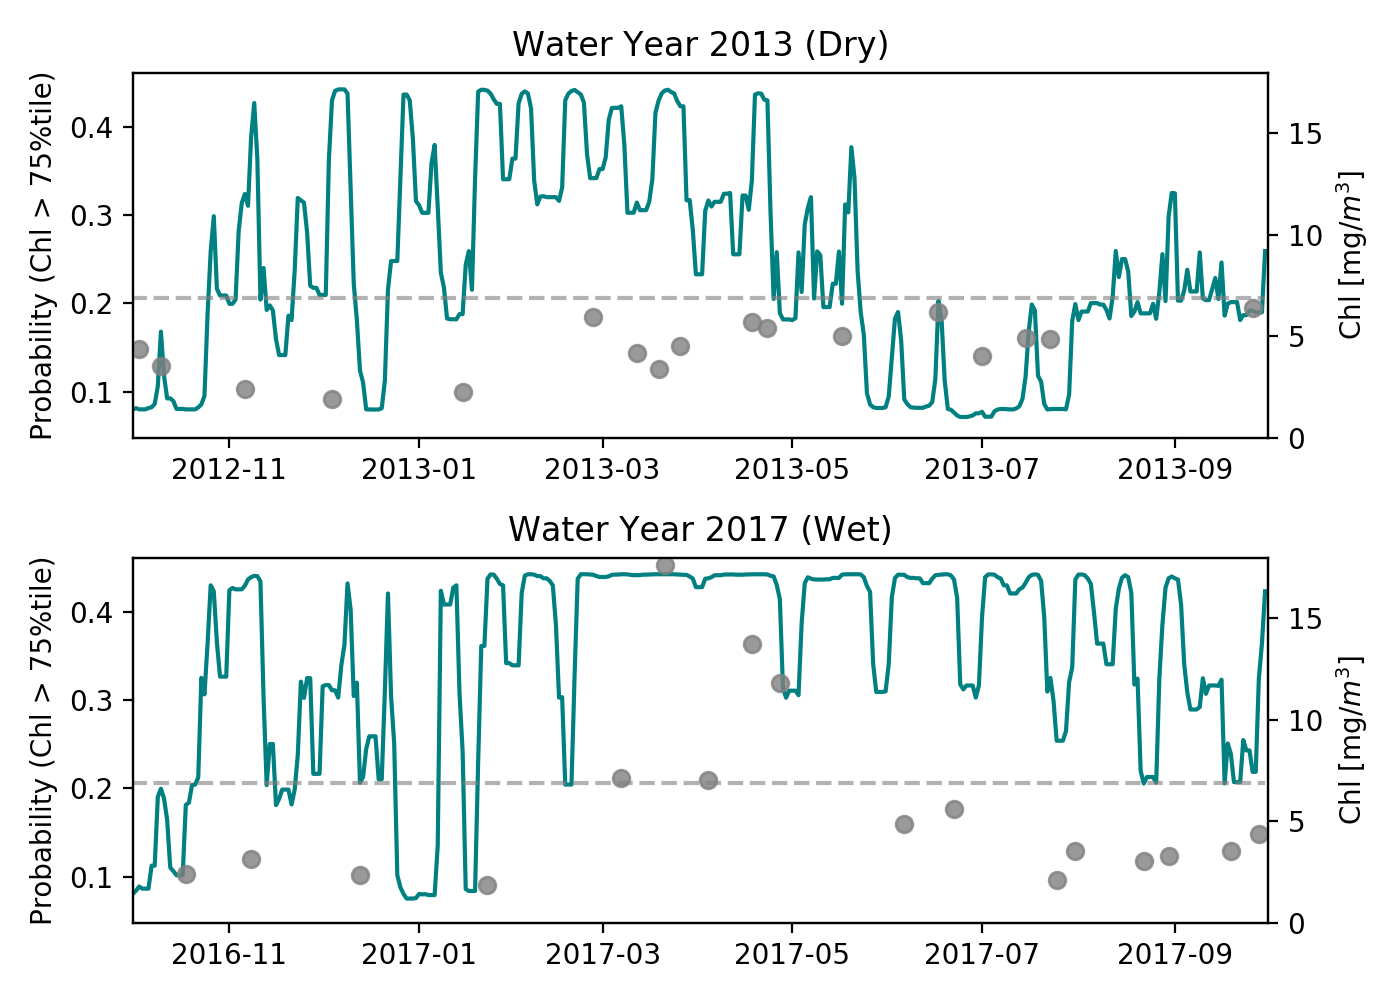
\includegraphics[width=0.8\textwidth]{Figures/probobability_chl_comparison.png}
\caption{Comparison of the probability of observing chlorophyll greater than the 0.75 chlorophyll quantile, given the modeled daily 3-day windowed \(Ri_x\) for water year 2013 and 2017, and chlorophyll observations. Chlorophyll data is averaged between USGS stations 24, 25, 27, and 29 for each day data is available. The solid blue lines show the probability, given by the left hand axis. The grey dots indicate chlorophyll observations, given by the right hand axis. Water year 2013 is given by the top figure and water year 2017 is given by the bottom figure.}
\label{fig:chl_comp}
\end{figure}
\FloatBarrier

\section{Discussion}\label{S:discussion}
The probabilistic method developed here is useful in its ability to utilize a relatively simple metric to calculate and predict the risk of phytoplankton blooms. It shows promise in successfully identifying periods of high likelihood of chlorophyll blooms which coincide with observed elevated levels of chlorophyll. While this method worked well identifying times during water year 2013 and 2017 when chlorophyll was elevated, work still needs to be done to understand what constitutes a relevant elevated probability. For example, in spring 2017, the probability of observing chlorophyll above the 0.75 quantile threshold is elevated and persists around 0.4 for several months. During this time, there were multiple. During the same seasonal period in 2013, the probability is elevated but more variable and is not consistently as high. For this period, chlorophyll is slightly elevated, but does not exceed the 0.75 quantile threshold. This difference suggests that sustained high probability periods matters in observing or that the relatively infrequent sampling could miss blooms events with shorter periods; however, more work needs to be done to make any conclusive conclusions. 

The data used to develop the probabilistic relationship between chlorophyll and \(Ri_x\) spanned 1990 - 2019. The 29 years of observations provide a large number of observations and visually provide a roughly log-normally distributed distribution of \(Ri_x\) (Fig. \ref{fig:rix_hist}). Despite having a long time record, there is still a lack of information in the tails of the distribution. While this distribution is likely sufficient in capturing the relationship between \(Ri_x\) and chlorophyll within the time range of 1990 - 2019, using this distribution for future conditions may need some more work. Lack of data on the tails of the distribution may underestimate the extremes, which are of particular interest in projected future conditions. Also, while the observed \(Ri_x\) historically appears to be relatively stationary, future conditions could shift the mean \(Ri_x\). 

The core assumption of the probabilistic calculations and analysis is that stratification caused by SIPS is the dominant control on phytoplankton dynamics. While there is evidence to support that this assumption is valid, there are also other processes that may be important. The deep channel, where the USGS data collected, is only a small portion of the entire bay. Shallow shoals make up most of the bay by area. These shoals have different dynamics due to their shallowness, and vertical stratification is much less significant while suspended sediment concentrations driven by wind and wave re-suspension are much more significant. These dynamics on the shoals can occur separate to the channel stratification processes and elevated chlorophyll levels on the shoal may not coincide with ideal channel chlorophyll conditions. In addition, mixing between the shoal and channel may play a non-trivial input of chlorophyll to the channel. This method would not capture these dynamics into predicting probabilities; however, this method may aid in understanding historical events. Using this method to calculate the likelihood of observing elevated chlorophyll conditions and comparing to chlorophyll observations may aid in identifying times when chlorophyll dynamics seem to fit within the stratification driven conceptual model and when other dynamics, such as shoal-channel mixing, may be important.   

While these results cannot be universally applied, some conclusions can be drawn about the implications of shifting stratification dynamics on phytoplankton blooms in SFB. The differences in the calculated probabilities of observing greater than the 0.75 and 0.9 quantiles of chlorophyll levels between 2013 and 2017 are striking (Fig. \ref{fig:prob_levels}). In 2017, these probabilities are elevated throughout the entire spring and summer, whereas the probabilities are elevated for a brief period in spring 2013 and then drop significantly. This difference, as well as observed chlorophyll levels, suggests that stratification dynamics played a role in chlorophyll dynamics. The conditions of these two years, particularly 2017, being proxies for projected extreme flow conditions suggest that under future scenarios stratification favorable conditions and subsequent phytoplankton blooms are likely expected.  

\section{Conclusions}\label{S:conclusion}
The probablistic method developed in this work successfully demonstrates a connection between chlorophyll and stratification dynamics by quantifying the likelihood of exceeding certain chlorophyll levels for observed stratification conditions. From this method, it is shown that high stratification periods (high \(Ri_x\)) have higher elevated chlorophyll level probabilities at all quantiles than low stratification periods (low \(Ri_x\)). This method was applied to two years of hydrodynamic model output, one serving as a dry year proxy and one serving as a wet year proxy. Calculated probabilities captured the observed chlorophyll dynamics and indicated strong differences between extreme wet and dry years, and suggesting that the likelihood of elevated chlorophyll levels will increase in extreme wet years. 

This method relies on several assumptions that limit the outcomes of the results and future applicability of the method; the observed relationship between \(Ri_x\) and chlorophyll observations is a stationary relationship, and that stratification is the dominant control on phytoplankton dynamics. These assumptions are reasonable for the purposes of the work presented in this paper; however, there are some limitations and issues to carefully consider in applying this method to other scenarios. Future work could explore more fully how stratification conditions might change under future scenarios through numerical modeling studies. In addition, more work needs to be done to understand how important and when are other processes, such as shoal-channel mixing, important in observed chlorophyll.

%% The Appendices part is started with the command \appendix;
%% appendix sections are then done as normal sections
%% \appendix

%% \section{}
%% \label{}

%% References
%%
%% Following citation commands can be used in the body text:
%% Usage of \cite is as follows:
%%   \cite{key}          ==>>  [#]
%%   \cite[chap. 2]{key} ==>>  [#, chap. 2]
%%   \citet{key}         ==>>  Author [#]

%% References with bibTeX database:

\bibliographystyle{model1-num-names}
\bibliography{bibliography.bib}

%% Authors are advised to submit their bibtex database files. They are
%% requested to list a bibtex style file in the manuscript if they do
%% not want to use model1-num-names.bst.

%% References without bibTeX database:

% \begin{thebibliography}{00}

%% \bibitem must have the following form:
%%   \bibitem{key}...
%%

% \bibitem{}

% \end{thebibliography}


\end{document}

%%
%% End of file `elsarticle-template-1-num.tex'.